\chapter{Introduction}

Quantum Computing is a promising field of research for computer scientists. In this context, the term ``quantum'' refers to the mathematical description of the physical phenomena of quantum mechanics as described in the 20th century by researchers like Werner Heisenberg, Erwin Schrödinger, Paul Dirac and John von Neumann. Quantum mechanics provide a mathematical framework that tries to cope with problems in the so-called classical physics theory, which turns out to have problems explaining phenomena on atomical scales. One of the first researchers who recognized the implications of the quantum mechanical approach on computer science was physicist Paul Benioff. In his paper, he described a ``microscopic quantum mechanical model of computers as represented by Turing machines''\cite{benioff1980computer}. Since the first description of such a computer, multiple approaches for quantum-aware computing machines were proposed. Two major contributions to this field are the so-called Adiabatic Quantum Computing and the \ac{QGM}. This thesis focuses on the implications of Shor's and Grover's algorithm on modern cryptography. Both algorithms are derived from the \ac{QGM} and weaken or even break important guarantees of commonly used cryptographic protocols. In the remainder of this thesis, these implications for the MACSec protocol suite are highlighted, and alternatives for a quantum-resistant variant are discussed and evaluated.

\section{Motivation}
The \ac{QGM} provides a mathematical description of a theoretical approach to build a quantum computer. This model uses qubits and logical ``quantum gates'' in analogy to bits and logical gates as used in classical computing theory. A single qubit is a two-dimensional vector that represents the state of this qubit. It is possible to transform a qubit's state by applying logical gates, represented by unitary matrices. Applying a logical gate is equivalent to ordinary matrix-vector multiplication of the qubit vector with the corresponding gate matrices. An algorithm in the \ac{QGM} consists of several qubits and a set of unitary matrices applied in a particular order. One of the first algorithms with a so-called quantum advantage over a classical algorithm was described by David Deutsch and Richard Josza and hence is often called the Deutsch-Josza algorithm. This algorithm computes whether a function \(f : \{0,1\}^n \rightarrow \{0, 1 \} \) is balanced or constant in a single iteration on a theoretical quantum computer\cite{deutsch1992rapid}. While this algorithm has mostly theoretical relevance to the field, different algorithms with a more practical approach were proposed in the last years. The Deutsch-Josza algorithm shows an essential property of practical quantum computers: Problems that are regarded as computationally too hard to solve on a classical computer may be solved efficiently by a quantum computer. One example of such a problem is the factorization of the product of two large prime numbers, which belongs to the complexity class NP and for which no polynomial-time solving algorithm is known. This specific problem was used to construct the RSA cryptosystem, developed by Rivest, Shamir and Adleman in 1978\cite{rivest1978method}. RSA is one of the most important and widely used cryptographic primitives in modern cryptographic protocols, and its secureness critically relies on the complexity of this problem. In 1999, Peter Shor proposed an algorithm for a quantum computer, built on the foundations of the quantum gate model, that factorizes large numbers in polynomial time on a quantum computer, using an implementation of the fast Fourier transformation. Shor even speculated that the quantum Fourier transformation could be used to speed up multiplication itself, resulting in lower asymptotical bounds for the time needed to break RSA on a quantum computer than performing the encryption on a classical computer.

Furthermore, Shor shows in his work how to apply the proposed quantum Fourier transformation to calculate the discrete logarithm \(x\) of a number \(m = g^x \bmod p\) in polynomial time. This variant can be used to break the security of the widely used discrete \ac{DH} public-key exchange and its variant \ac{ECDH}\cite{shor1999polynomial}. \ac{DH}-based protocols have gained significant importance in the last years and even superseded RSA-based key exchanges in many cases. An example is the widely used TLS protocol, which in its recent 1.3 version completely dropped support for RSA-based key exchanges in favor of \ac{DH} and \ac{ECDH}-based approaches.

\begin{figure}[ht]
    \centering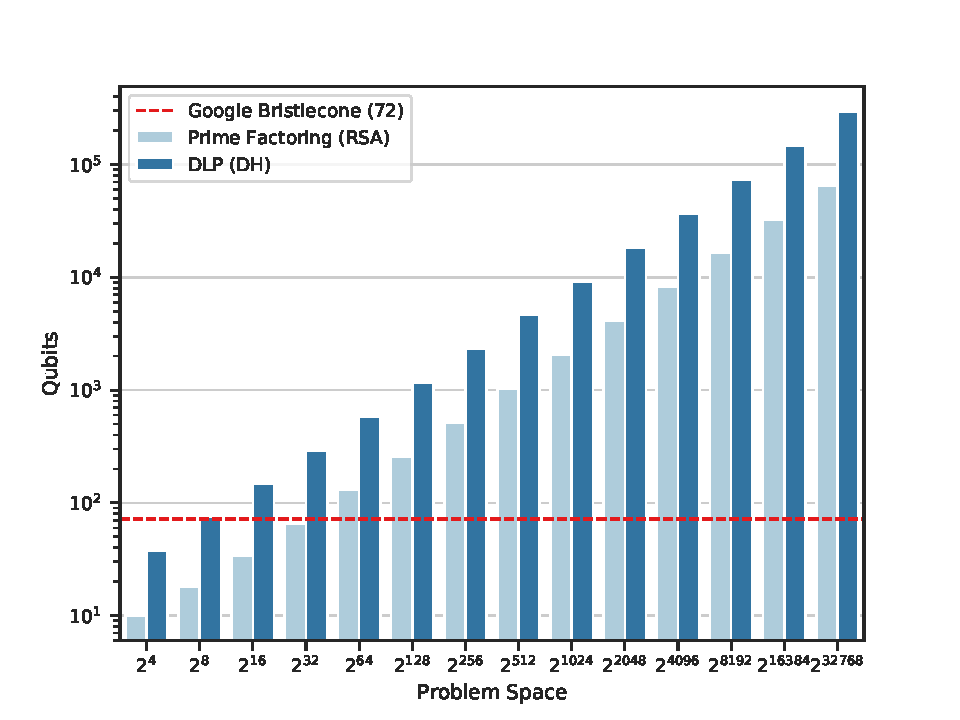
\includegraphics[width=1.0\linewidth]{plot_line_shor_rsa.pdf}
    \caption{Estimates of the number of qubits needed to break an RSA/ECC problem of a certain size. The y-axis is logarithmic to a base of two. The estimated number for breaking an RSA key of \(2^n\) is \(2n+2\), according to \cite{haner2017factoring}. For an ECC \ac{DLP} of size \(2^n\) the number is \(9n+2\ln(n)\), according to \cite{roetteler2017quantum}. The dotted, red line shows the amount of currently available physical qubits supported by Google's Bristlecone architecture (\(72\)).}\label{fig:shor_vs_rsa_dlog}
\end{figure}


Lov Grover proposed another important algorithm in 1996\cite{grover1996fast}. Grover described a quantum mechanical algorithm for searching a key in an unsorted database with \(n \) elements. The proposed algorithm has a runtime of \(\bigo(\sqrt{n})\) as opposed to a classical algorithm that needs to take \(\bigo(n)\) steps, given the number of elements. This algorithm is also of particular interest to the cryptographic community since the best-known approach for many symmetrical cryptosystems is a brute force attack, which can be reduced on a random search in the keyspace of the symmetrical cipher. For symmetrical keys with size \(2^n \), the search space is therefore effectively halved by Grover's algorithm.

Both algorithms were already implemented in real-world experimental setups. In 2001 Vandersypen et al. factored the number 15 by implementing Shor’s algorithm on a quantum computer\cite{vandersypen2001experimental}. Due to limitations in the practical realization of sufficient large quantum computers, as of today, there is no realistic scenario where Shor's algorithm can be used to break state-of-the-art encryption in the next decade. Figure~\ref{fig:shor_vs_rsa_dlog} shows an overview of how many qubits are needed to break a cryptosystem of a specific size alongside the number of available qubits on Google's Bristlecone Architecture, one of the largest quantum computer implementations available today. The number of needed and available qubits are specified as ``physical'' qubits, meaning that the number of available qubits on a single quantum computer may be smaller, while the number of needed ``logical'' qubits to break a particular key may be magnitudes of order higher. The main reason is the need for error correction. Even in the optimistic scenario with no need for error correction, as of today, no available quantum computer is close to breaking any encryption scheme with a reasonable key size. However, in the last years, an ever-growing effort was put into building a more capable quantum computer. While it is difficult to compare such systems directly, a standard measure is the number of coherent qubits realized. In cooperation with Oak Ridge National Laboratory and Google, the \ac{NASA} was recently able to show so-called ``quantum supremacy'' or ``quantum advantage'' on a quantum computer design that uses 54 qubits\cite{arute2019quantum}. While this number and other properties like coherence time on these machines may be magnitudes of orders too small for a practical application, an exponential development of these parameters, similar to Moore's law, must be assumed. The issue gets even more pressing when considering that governmental agencies may already be storing large amounts of encrypted data in specially tailored data centers for later decryption.\footurl{https://www.wired.com/2012/03/ff-nsadatacenter/} This renders currently used cryptographic systems unusable for future applications and raises the need for two important tasks: Finding new algorithms that rely on different problems and provide better resistance against attackers with access to a sufficiently large quantum computer and second, identify currently used protocols and system which rely on cryptographic protocols that are known to be vulnerable against such attackers and securing them against quantum-adversary.

One class of protocols heavily used to encrypt and authenticate data streams are so-called \ac{VPN} protocols. \acp{VPN} are commonly used to span a virtual, encrypted network link between two, often geographically separated networks. These connections are virtual in the sense that for the computing equipment in such networks, it looks like they reside in the same \ac{LAN} while the network traffic is transmitted over different public network links. Encryption schemes are used in such protocols to keep the transmitted data confidential, even during transmission over untrusted lines. Solutions like IPSEC\cite{rfc4301}, OpenVPN\footurl{https://openvpn.net/} and Wireguard\footurl{https://www.wireguard.com/} are commonly used to connect IP-Layer network links, while protocols like MACSec as defined by IEEE 802.1AE\cite{IEEE8021AE} are used to connect two nodes in the same \ac{LAN} directly. MACSec is often used in places like carrier-grade interconnects where control over the physical link itself may not be possible. Due to the amount of data usually transmitted over such links and the broad number of subscribers, a single carrier can be the bottleneck for data and, as such, can be of particular interest to an attacker. This may be even further relevant in the context of \ac{PQ} security when taking into account that the first sufficient large quantum computers are probably going to be owned by large organizations, which are likely also have the resources to access such network interconnects directly.

\section{Problem Statement}
This thesis is part of the QuaSiModO project\footurl{https://www.pq-vpn.de/index.html} and focuses on the 802.1X and 802.1AE protocol suites provided by the \ac{IEEE}. Cryptographic schemes are an essential part of this wieldy employed protocol suite, used for authentication and encryption in wired, as well as in wireless networks. This thesis aims to identify used cryptographic protocols and an evaluation of their vulnerability to attackers with a (theoretical) sufficient large quantum computer. Currently, a broad range of post-quantum algorithms is available. It is crucial to not only select an arbitrary alternative but to evaluate their performance regarding the protocol's design goals and select a candidate, which allows for a future proof design that can be used as a drop-in replacement. Optimally, a replacement should ensure security against quantum adversaries and additionally keep into account that computing resources may be constrained.

\section{Methodology}
In Chapter~2, an overview of the details of the used technologies and protocols is provided. It covers the \ac{IEEE} 802.1X and 802.1AE protocol suites and provides an overview of quantum computing with a particular focus on \ac{PQC}. Furthermore, an overview of work related to this field is provided. Chapter 3 defines requirements for a PQ implementation of the 802.1X protocol suite, depending on used cryptographic algorithms in 802.1X and limitations from the used Ethernet layer. The fourth chapter focuses on a design proposal of a quantum-resistant implementation of the 802.1X protocol. Available alternatives to the used cryptographic schemes shall be evaluated, and a proposal to harden the protocol suite shall be provided. This thesis does explicitly not aim to employ new quantum-resistant cryptographic schemes but rather evaluates existing schemes and selects them to fit the requirements that arise from the characteristics of the concerned protocols. The selection of the cryptographic protocols is tightly coupled to an ongoing project, hosted by the \ac{NIST}, that aims to ``solicit, evaluate, and standardize one or more quantum-resistant public-key cryptographic algorithms''\footurl{https://csrc.nist.gov/projects/post-quantum-cryptography}. Vulnerable components of the protocol are outlined, and appropriate countermeasures are provided. The fifth chapter focuses on an experimental evaluation of the proposed design.

\endinput